% Created 2023-03-06 lun 21:22
% Intended LaTeX compiler: pdflatex
\documentclass[aspectratio=169, usenames,svgnames,dvipsnames]{beamer}
\usepackage[utf8]{inputenc}
\usepackage[T1]{fontenc}
\usepackage{graphicx}
\usepackage{longtable}
\usepackage{wrapfig}
\usepackage{rotating}
\usepackage[normalem]{ulem}
\usepackage{amsmath}
\usepackage{amssymb}
\usepackage{capt-of}
\usepackage{hyperref}
\usepackage{color}
\usepackage{listings}
\usepackage{mathpazo}
\usepackage{gensymb}
\usepackage{amsmath}
\usepackage{diffcoeff}
\usepackage{steinmetz}
\usepackage{mathtools}
\usepackage{fancyvrb}
\DefineVerbatimEnvironment{verbatim}{Verbatim}{fontsize=\tiny, formatcom = {\color{black!70}}}
\bibliographystyle{plain}
\usepackage{siunitx}
\sisetup{per-mode=symbol}
\sisetup{output-decimal-marker={,}}
\DeclareSIUnit{\watthour}{Wh}
\DeclareSIUnit{\wattpeak}{Wp}
\DeclareSIUnit{\watthour}{Wh}
\DeclareSIUnit{\amperehour}{Ah}
\usepackage{steinmetz}
\hypersetup{colorlinks=true, linkcolor=Blue, urlcolor=Blue}
\usepackage[symbol, perpage]{footmisc}
\parskip=5pt
\usetheme{Boadilla}
\usecolortheme{rose}
\usefonttheme{serif}
\author{\href{https://oscarperpinan.github.io}{Oscar Perpiñán Lamigueiro}}
\date{}
\title{SFCR: Seguridad Eléctrica}
\institute[UPM]{Universidad Politécnica de Madrid}
\setbeamercolor{alerted text}{fg=blue!50!black} \setbeamerfont{alerted text}{series=\bfseries}
\AtBeginSubsection[]{\begin{frame}[plain]\tableofcontents[currentsubsection,sectionstyle=show/hide,subsectionstyle=show/shaded/hide]\end{frame}}
\AtBeginSection[]{\begin{frame}[plain]\tableofcontents[currentsection,hideallsubsections]\end{frame}}
\beamertemplatenavigationsymbolsempty
\setbeamertemplate{footline}[frame number]
\setbeamertemplate{itemize items}[triangle]
\setbeamertemplate{enumerate items}[circle]
\setbeamertemplate{section in toc}[circle]
\setbeamertemplate{subsection in toc}[circle]
\hypersetup{
 pdfauthor={\href{https://oscarperpinan.github.io}{Oscar Perpiñán Lamigueiro}},
 pdftitle={SFCR: Seguridad Eléctrica},
 pdfkeywords={},
 pdfsubject={},
 pdfcreator={Emacs 28.2 (Org mode 9.6)}, 
 pdflang={Spanish}}
\begin{document}

\maketitle


\section{Definiciones}
\label{sec:orgc43f254}

\begin{frame}[label={sec:org06732fa}]{Contacto Directo e Indirecto}
\begin{description}
\item[{Partes Activas:}] Conductores y piezas conductoras bajo tensión en
servicio normal. Incluyen el conductor neutro y las partes
conectadas a él.

\item[{Contacto Directo:}] contacto de personas o animales con partes
activas de los materiales y equipos

\item[{Contacto Indirecto:}] contacto de personas o animales con partes que
se han puesto bajo tensión como resultado de un fallo de aislamiento.
\end{description}
\end{frame}

\begin{frame}[label={sec:orge6107a8}]{Masa y Tierra}
\begin{description}
\item[{Masa:}] Conjunto de las partes metálicas de un aparato que, en
condiciones normales, están aisladas de las partes activas.

\item[{Tierra:}] Masa conductora de la tierra en la que el potencial
eléctrico en cada punto se toma, convencionalmente, igual a cero.

\item[{Toma de tierra:}] Electrodo, o conjunto de electrodos, en contacto
con el suelo y que asegura la conexión eléctrica con el mismo.
\end{description}
\end{frame}

\begin{frame}[label={sec:orge2a47d9}]{Tensión de contacto y defecto}
\begin{block}{Tensión de contacto}
\begin{itemize}
\item Tensión que aparece entre \alert{partes accesibles simultáneamente} al
ocurrir un fallo de aislamiento.
\item Termino empleado en protección contra contactos indirectos.
\end{itemize}
\end{block}

\begin{block}{Tensión de defecto}
\begin{itemize}
\item Tensión que aparece a causa de un defecto de aislamiento, entre dos
masas, entre una masa y un elemento conductor, o entre una masa y
una toma de tierra de referencia.
\end{itemize}
\end{block}
\end{frame}

\begin{frame}[label={sec:org3d77d8d}]{Clases de materiales}
\begin{itemize}
\item Material de clase 0
\begin{itemize}
\item La protección se basa en el aislamiento principal
\end{itemize}
\item Material de clase I
\begin{itemize}
\item La protección se basa en el aislamiento principal \alert{y}  en conexión de las partes conductoras accesibles a un conductor de
protección puesto a tierra
\item Las partes conductoras accesibles no pueden presentar tensiones peligrosas.
\end{itemize}
\item Material de clase II
\begin{itemize}
\item La protección incluye doble aislamiento o aislamiento reforzado.
\item No requieren la utilización de puesta a tierra para la protección
\item No dependen de las condiciones de la instalación.
\end{itemize}
\item Material de clase III
\begin{itemize}
\item La protección se basa en la alimentación a muy baja tensión (tensiones inferiores a 50 V en c.a. ó a 75V en c.c.)
\end{itemize}
\end{itemize}
\end{frame}

\begin{frame}[label={sec:org471a3cc}]{Esquemas de conexión a tierra}
\begin{description}
\item[{Primera letra:}] conexión de alimentación y tierra

\begin{description}
\item[{T=}] conexión directa de un punto de alimentación a tierra

\item[{I=}] aislamiento de todas las partes activas respecto a tierra
\end{description}

\item[{Segunda letra:}] conexión de masas con tierra

\begin{description}
\item[{T=}] masas conectadas directamente a tierra

\item[{N=}] masas conectadas directamente a punto de alimentación puesto
a tierra (en alterna, normalmente el neutro)
\end{description}
\end{description}
\end{frame}

\begin{frame}[label={sec:org81029e5}]{Esquemas de conexión a tierra}
\begin{description}
\item[{TN:}] en alterna, neutro puesto a tierra, y masas conectadas al
neutro (directamente o a través de un conductor de protección).

\item[{TT:}] en alterna, neutro puesto a tierra y masas a tierra, pero de
forma independiente.\\[0pt]
\emph{Instalaciones receptoras en una red de distribución pública de BT}

\item[{IT:}] todos los conductores activos aislados de tierra, y masas
conectadas a tierra.\\[0pt]
\emph{Esquema habitual en zona del generador FV en SFCR europeos}
\end{description}
\end{frame}

\begin{frame}[label={sec:org86bac07}]{Esquemas de conexión a tierra}
En un sistema fotovoltaico es de uso común que el esquema de tierra sea:
\begin{itemize}
\item \alert{IT en la zona del generador fotovoltaico}
\item \alert{TT a partir de la salida del inversor}.
\end{itemize}
\end{frame}

\section{Protección de las personas}
\label{sec:orgc1fac9c}

\subsection{Efectos de la corriente eléctrica}
\label{sec:org82fbe3a}

\begin{frame}[label={sec:org75baf36}]{Intensidad y tiempo de contacto}
\begin{itemize}
\item Hasta 10 mA no genera efectos peligrosos (calambres).

\item Por encima de 500 mA puede producir fibrilación muscular.

\item La \alert{intensidad} que circula \alert{depende de la tensión de contacto y la
resistencia expuesta}.

\begin{itemize}
\item Reducir tensión.

\item Aumentar resistencia (guantes, calzado, aislamiento del suelo)
\end{itemize}
\end{itemize}
\end{frame}

\begin{frame}[label={sec:org2c36c16}]{Frecuencia eléctrica}
\begin{itemize}
\item Continua:

\begin{itemize}
\item Umbral de percepción: 2 mA

\item Umbral control muscular: 75 mA

\item Menos peligrosa que alterna convencional. Puede producir
electrolisis de la sangre.
\end{itemize}

\item Alterna 50 Hz:

\begin{itemize}
\item Umbral de percepción: 0.5 mA

\item Umbral de control muscular: 15 mA
\end{itemize}

\item Alterna 10 kHz:

\begin{itemize}
\item Umbral de percepción: 5 mA

\item Umbral de control muscular: 75 mA

\item Debido al efecto pelicular, los efectos son menores que la alterna
convencional (la corriente circula por la piel, sin atravesar
órganos internos).
\end{itemize}
\end{itemize}
\end{frame}

\subsection{Contacto Directo}
\label{sec:org168dd7c}

\begin{frame}[label={sec:org1f817dd}]{REBT: Contactos Directos}
Según la ITC-BT-24 las protecciones a utilizar para proteger frente a
contactos directos deben estar \alert{basadas en evitar que una persona pueda
entrar en contacto con las partes activas} de la instalación.

\begin{itemize}
\item Protección por \alert{aislamiento de las partes activas}

\item Protección por medio de \alert{barreras o envolventes}

\item Protección por medio de \alert{obstáculos}

\item Protección por puesta \alert{fuera de alcance} por alejamiento

\item Protección complementaria por \alert{dispositivos de corriente
diferencial}-residual
\end{itemize}
\end{frame}


\begin{frame}[label={sec:orgdc2be74}]{Contacto Directo IT}
\begin{center}
\includegraphics[height=0.5\textheight]{../figs/ContactoDirectoIT_Capacidad.pdf}
\end{center}

$$I_{f}\leq100\, mA\Longrightarrow R_{iso}\geq10\cdot V_{ocG}-R_{H}$$

Se necesitan tensiones de generador superiores a los \(\SI{1000}{\volt}\)
para producir dolor, y tensiones superiores a los \(\SI{3000}{\volt}\)
para que exista riesgo por fibrilación.
\end{frame}

\begin{frame}[label={sec:org5922337}]{Contacto Directo TT}
$$I_{F,max}=\frac{V_{ocG}}{R_{H}+R_{p}+R_{ts}}$$

\begin{columns}
\begin{column}{0.5\columnwidth}
\begin{center}
\includegraphics[height=0.5\textheight]{../figs/ContactoDirectoTT.pdf}
\end{center}
\end{column}

\begin{column}{0.5\columnwidth}
\begin{center}
\includegraphics[height=0.5\textheight]{../figs/ContactoDirectoTT_simple.pdf}
\end{center}
\end{column}
\end{columns}
\end{frame}




\subsection{Contacto Indirecto}
\label{sec:orge9d4095}


\begin{frame}[label={sec:org4aab444}]{REBT: Contactos Indirectos}
La ITC-BT-24 recoge las formas de protección para contactos
indirectos:

\begin{itemize}
\item Protección por \alert{corte automático de la alimentación}: cuando se
produce el contacto, el objetivo es evitar que la fuente eléctrica
siga alimentando la fuga.

\item Protección por empleo de \alert{equipos de clase II o por aislamiento
equivalente}, con la misión de alcanzar resistencias de aislamiento
de alto valor y estables en el tiempo.

\item \alert{Puesta a tierra}, como camino preferente para conducir la corriente
de fuga y para servir de potencial común para todos los elementos que
entran en contacto con ella.
\end{itemize}
\end{frame}

\begin{frame}[label={sec:orgc089842}]{Contacto Indirecto IT}
\begin{columns}
\begin{column}{0.5\columnwidth}
\begin{center}
\includegraphics[height=0.5\textheight]{../figs/ContactoIndirectoIT.pdf}
\end{center}

$$\begin{aligned}
V_{c} & = & 0\\
I_{F} & = & 0\end{aligned}$$
\end{column}

\begin{column}{0.5\columnwidth}
\begin{center}
\includegraphics[height=0.9\textheight]{../figs/ContactoIndirectoIT_simple.pdf}
\end{center}
\end{column}
\end{columns}
\end{frame}


\begin{frame}[label={sec:orgfb26e6c}]{Contacto Indirecto TT}
\begin{columns}
\begin{column}{0.5\columnwidth}
\begin{center}
\includegraphics[height=0.5\textheight]{../figs/ContactoIndirectoTT.pdf}
\end{center}
$$V_{c}\simeq I_{scG}\cdot R_{tp}$$
\end{column}

\begin{column}{0.5\columnwidth}
\begin{center}
\includegraphics[height=0.9\textheight]{../figs/ContactoIndirectoTT_simple.pdf}
\end{center}
\end{column}
\end{columns}
\end{frame}


\subsection{Niveles de Protección en Sistema IT}
\label{sec:orgf2592d3}


\begin{frame}[label={sec:org4350c60}]{Tres niveles de protección}
Todo el sistema de protección para sistemas IT se puede concebir en tres
niveles:

\begin{itemize}
\item Nivel 1: Refuerzo del aislamiento de las partes activas.

\item Nivel 2: Sistema de detección de aislamiento.

\item Nivel 3: Puesta a tierra.
\end{itemize}
\end{frame}

\begin{frame}[label={sec:org9d46dd5}]{Nivel 1: Refuerzo del aislamiento de las partes activas.}
\begin{description}
\item[{Configuración flotante del generador:}] se imposibilitan los
accidentes por la aparición de contactos indirectos de primer
contacto.

\item[{Cableado con aislamiento de protección:}] Estos aislamientos
refuerzan la protección contra contactos indirectos.

\item[{Aislamiento galvánico AC-DC:}] Mediante transformadores de devanados
independientes en los inversores se imposibilita el cierre de
corriente de fallo a través del inversor.
\end{description}
\end{frame}

\begin{frame}[label={sec:org068a323}]{Nivel 2: Sistema de detección de aislamiento.}
\begin{description}
\item[{Vigilante de aislamiento:}] Este elemento genera una señal de baja
frecuencia (2 a 5 Hz) para evitar las fugas capacitivas del cableado,
y que inyecta en un polo activo midiendo la corriente de retorno, y
por tanto, la resistencia de aislamiento.

\item[{En caso de pérdida de aislamiento,}] el vigilante ordena el
disparo de los interruptores aislando el campo fotovoltaico
afectado. Idealmente activa el cortocircuito del campo y la puesta a
tierra del mismo.
\end{description}
\end{frame}

\begin{frame}[label={sec:org71e3f89}]{Nivel 3: Protección en caso de fallo de los niveles 1 y 2:}
\begin{description}
\item[{En caso de fallo de los niveles anteriores}] aún queda la
protección proporcionada por la puesta a tierra directa de todas las
masas de la planta. Gracias a ella se limitará la tensión que con
respecto a tierra puedan adquirir las masas en caso de derivación.
\end{description}
\end{frame}



\section{Protección de los equipos}
\label{sec:org1bf9ebe}

\subsection{Tormentas eléctricas}
\label{sec:org391965a}

\begin{frame}[label={sec:org7becc91}]{Formación de las tormentas}
\begin{columns}
\begin{column}{0.5\columnwidth}
\begin{center}
\includegraphics[width=0.9\textwidth]{../figs/FormacionTormenta.pdf}
\end{center}
\end{column}

\begin{column}{0.5\columnwidth}
\begin{itemize}
\item Dentro de los núcleos tormentosos se producen campos eléctricos.

\item Cuando el campo eléctrico interno de la nube alcanza la ruptura del
aire, se producen descargas eléctricas.

\item \alert{Esta descarga comienza en la nube} con un \alert{trazador descendente} hacia
la superficie terrestre.

\item Trazadores ascendentes surgen cuando el descendente se acerca a
10-100 m de la superficie terrestre.

\item Aquel trazador ascendente que conecta con el descendente cierra la
descarga y determina el lugar del impacto.
\end{itemize}
\end{column}
\end{columns}
\end{frame}

\begin{frame}[label={sec:org88671a7}]{Influencia de las condiciones locales}
\begin{columns}
\begin{column}{0.5\columnwidth}
\begin{center}
\includegraphics[width=0.9\textwidth]{../figs/FormacionTormenta.pdf}
\end{center}
\end{column}

\begin{column}{0.5\columnwidth}
\begin{itemize}
\item \alert{La descarga está determinada principalmente por el campo eléctrico
interno de la nube}, con una menor influencia debida a las
condiciones de la superficie terrestre.

\item Las \alert{condiciones locales sólo influyen} a distancias de 10-100 metros.

\item Las \alert{construcciones metálicas de mayor altura} (antenas) o superficie
(instalaciones fotovoltaicas) favorecen la formación de trazadores
ascendentes que conecten con el descendente.
\end{itemize}
\end{column}
\end{columns}
\end{frame}

\begin{frame}[label={sec:org4a263af}]{Influencia de los sistemas fotovoltaicos}
Por tanto, \alert{las instalaciones fotovoltaicas no aumentan la probabilidad
de descargas locales} (determinadas por las nubes), pero una vez que se
producen, son lugares con mayor probabilidad de impacto.
\end{frame}

\begin{frame}[label={sec:org120d51b},plain]{Descarga y campo magnético}
\begin{columns}
\begin{column}{0.4\columnwidth}
\begin{center}
\includegraphics[height=0.8\textheight]{../figs/SobretensionInducida.pdf}
\end{center}
\end{column}
\begin{column}{0.6\columnwidth}
\begin{itemize}
\item Una descarga eléctrica supone una \alert{corriente de gran valor} en un lapso de \alert{tiempo muy corto}.

\item Esta corriente produce una \alert{inducción magnética} a su alrededor de caracter \alert{variable}.

\item Un flujo magnético variable produce una \alert{fuerza electromotriz} entre los extremos del área atravesada.
\end{itemize}
\end{column}
\end{columns}
\end{frame}

\begin{frame}[label={sec:orgac4a9dc},plain]{Factores de influencia}
\begin{columns}
\begin{column}{0.4\columnwidth}
\begin{center}
\includegraphics[height=0.8\textheight]{../figs/SobretensionInducida.pdf}
\end{center}
\end{column}
\begin{column}{0.6\columnwidth}
La fuerza electromotriz inducida depende de:

\begin{itemize}
\item \alert{Valor de la inducción magnética} (depende de la tormenta).

\item \alert{Distancia} de la descarga al sistema (depende principalmente de la
tormenta).

\item \alert{Area efectiva del sistema} (depende del diseñador y del instalador).
\end{itemize}
\end{column}
\end{columns}
\end{frame}

\subsection{Protecciones}
\label{sec:org055a1bd}


\begin{frame}[label={sec:org071d882}]{Area y cableado}
\begin{center}
\includegraphics[width=\textwidth]{../figs/BucleCableadoOptimo.pdf}
\end{center}
\end{frame}

\begin{frame}[label={sec:orgcb0c1a4}]{Protección externa}
Un sistema de protección externa contra el rayo se compone de:

\begin{itemize}
\item Terminal aéreo (punta)

\item Conductor(es) de bajada (interconectados)

\item Puesta a tierra.
\end{itemize}
\end{frame}

\begin{frame}[label={sec:org0db80d3}]{Protección externa}
\begin{center}
\includegraphics[height=0.9\textheight]{../figs/AreaProteccionPararrayos.pdf}
\end{center}
\end{frame}

\begin{frame}[label={sec:org419465d}]{Protección externa}
\begin{itemize}
\item Se debe calcular una \alert{distancia de seguridad} entre la bajada del
pararrayos y las instalaciones metálicas cercanas.

\begin{itemize}
\item Se asume que una distancia mayor a 1 metro es superior a la distancia
de seguridad.
\end{itemize}

\item \alert{Si la distancia es inferior a la de seguridad}, el sistema de puesta
a tierra de la protección externa y la estructura metálica deben
\alert{interconectarse} para evitar la existencia de descargas entre
conductores.

\item \alert{Si la distancia es superior a la de seguridad}, los sistemas de
puesta a tierra deben ser \alert{independientes}.
\end{itemize}
\end{frame}

\begin{frame}[label={sec:org50e6cfc}]{Protecciones internas}
\begin{itemize}
\item \alert{Todas las masas deben estar conectadas a un sistema de puesta a
tierra}.

\item En la entrada/salida de cada elemento a proteger se instalan
\alert{supresores de tensión (varistores)} entre conductores activos y
tierra.
\end{itemize}
\end{frame}

\section{Resumen de protecciones}
\label{sec:org7504087}

\begin{frame}[label={sec:org328d8c2},plain]{Diagrama Unifilar}
\begin{center}
\includegraphics[width=1\textwidth]{../figs/UnifilarCR1.pdf}
\end{center}
\end{frame}

\subsection{Circuito DC}
\label{sec:org121dc16}
\begin{frame}[label={sec:org882849e}]{}
\begin{center}
\includegraphics[height=0.8\textheight]{../figs/CajaProteccionesPhotocampa.pdf}
\end{center}
\end{frame}


\begin{frame}[label={sec:org6f7c91f}]{Cortocircuitos}
\begin{itemize}
\item El \alert{cortocircuito} es un punto de trabajo \alert{no peligroso para el
generador fotovoltaico}.

\item El cortocircuito puede, sin embargo, ser \alert{perjudicial para el
inversor}. Como medio de protección se incluyen fusibles de tipo gG
normalizados según EN 60269 en cada polo.

\item Para las personas es \alert{peligrosa la realización o eliminación de un
cortocircuito franco en el campo generador}, por la posibilidad de
que se establezca un arco eléctrico.

\item Es recomendable la \alert{conducción separada} del positivo y del negativo
para evitar cortocircuitos por pérdida de aislamiento.
\end{itemize}
\end{frame}

\begin{frame}[label={sec:org73d3fc1}]{Fusibles}
\begin{itemize}
\item El \alert{fusible por rama} sirve principalmente como \alert{elemento de
seccionamiento} (facilita las tareas de mantenimiento).

\item Suele utilizarse \(I_{n} \geq 1.25\cdot I_{scG}\)

\item La corriente de activación es \(I_{2}=1.6\cdot I_{n}\)
\end{itemize}

\begin{columns}
\begin{column}{0.5\columnwidth}
\begin{center}
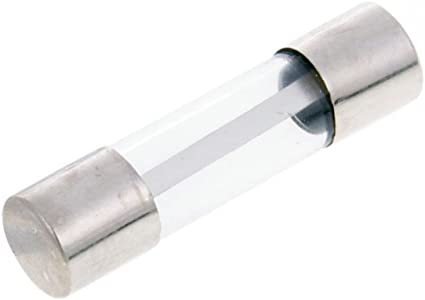
\includegraphics[height=0.4\textheight]{../figs/fusible.jpg}
\end{center}
\end{column}


\begin{column}{0.5\columnwidth}
\begin{center}
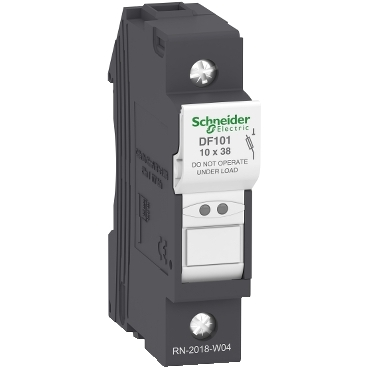
\includegraphics[height=0.5\textheight]{../figs/portafusible.JPG}
\end{center}
\end{column}
\end{columns}
\end{frame}

\begin{frame}[label={sec:org4fc3a64}]{Descargadores de tensión}
\begin{itemize}
\item Entrada CC del inversor protegida mediante \alert{descargadores de tensión} para
proteger contra sobretensiones de origen atmosférico.

\item Tensión de operación marcada por el diseño del sistema concreto,
entre la menor tensión en el punto de máxima potencia y la mayor
tensión de circuito abierto.

\begin{center}
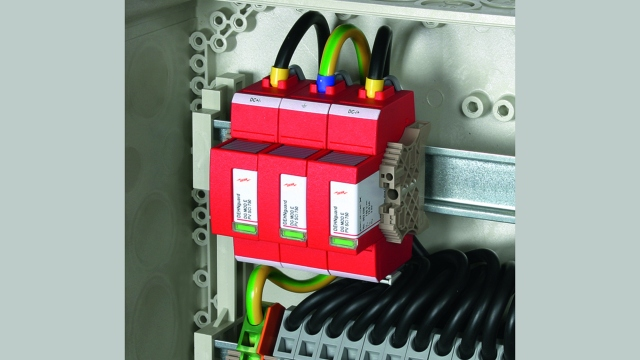
\includegraphics[height=0.5\textheight]{../figs/varistorDEHN.jpg}
\end{center}
\end{itemize}
\end{frame}


\subsection{Circuito AC}
\label{sec:org72cc39c}
\begin{frame}[label={sec:org3ba932f}]{}
\begin{center}
\includegraphics[height=0.9\textheight]{../figs/CajaAC.jpg}
\end{center}
\end{frame}

\begin{frame}[label={sec:org3cccd2f}]{Cortocircuitos y sobrecargas}
\begin{itemize}
\item Es necesario incluir un \alert{interruptor general manual} (interruptor
magnetotérmico omnipolar)

\begin{itemize}
\item Ubicado en el cuadro de contadores de la instalación fotovoltaica,
\alert{accesible sólo a la empresa distribuidora}.
\end{itemize}

\item Un \alert{segundo magnetotérmico omnipolar} (de menor intensidad nominal)
actuará antes que el interruptor general manual, salvo
cortocircuitos de cierta importancia provenientes de la red de la
compañía.

\item Recomendable un magnetotérmico de menor corriente para cada
inversor.
\end{itemize}
\end{frame}

\begin{frame}[label={sec:org2508242}]{Cortocircuitos y sobrecargas}
\begin{itemize}
\item Se utilizarán \alert{magnetotérmicos tipo C} (indicados cuando no existen corrientes de arranque de consumo elevadas).

\item Su corriente de activación es \(I_{2}=1.45\cdot I_{n}\).
\end{itemize}
\end{frame}

\begin{frame}[label={sec:org7d24d05}]{Interruptor diferencial}
\begin{itemize}
\item \alert{No funciona en circuitos DC} (alternativa: vigilante de
aislamiento).

\item Se debe incluir un diferencial de 30 mA con corriente nominal
superior a la del magnetotérmico de protección.

\item El diferencial \alert{no protege el tramo comprendido entre él y el punto
de conexión a red} (conexión TT).
\end{itemize}
\begin{center}
\includegraphics[height=0.3\textheight]{../figs/InterruptorDiferencial.pdf}
\end{center}
\end{frame}



\begin{frame}[label={sec:org463ecf8}]{Puesta a tierra}
\begin{itemize}
\item \alert{La puesta a tierra} se realizará de forma que \alert{no altere la de la
compañía eléctrica distribuidora}, con el fin de no transmitir
defectos a la misma.

\item \alert{Las masas de la instalación fotovoltaica estarán conectadas a una
tierra independiente de la del neutro} de la empresa distribuidora
de acuerdo con el Reglamento Electrotécnico para Baja Tensión.
\end{itemize}
\end{frame}


\section{Puesta a tierra}
\label{sec:org147c47b}

\begin{frame}[label={sec:org587b5e1}]{Tomas de tierra existentes}
A la hora de realizar puestas a tierra en lugares donde ya existen
tomas a tierra que pertenecen a otras instalaciones eléctricas.

\begin{itemize}
\item Cuando corresponda a la \alert{instalación de Baja Tensión del edificio}
\alert{se utilizará la puesta a tierra existente} para conectar las masas
del sistema fotovoltaico.

\item Cuando corresponde al \alert{neutro de Media Tensión del transformador de
la compañía eléctrica} es necesario \alert{separarse suficientemente} para
no interferir en su funcionamiento. Para terrenos de resistividad no
elevada (\(\rho<\SI{100}{\ohm\meter}\)), esta condición se cumple para
distancias superiores a \(\SI{15}{\meter}\).
\end{itemize}
\end{frame}


\begin{frame}[label={sec:org7611a27}]{Cálculo de resistencia para generador}
\begin{itemize}
\item Un sistema IT es intrínsecamente seguro.
\item No obstante, la corriente de defecto máxima es \(I_f=\SI{30}{\milli\ampere}\) (vigilante de aislamiento).
\item El sistema de puesta a tierra garantizará que cualquier masa no pueda dar lugar a tensiones de contacto superiores a \(V_{max}=\SI{24}{\volt}\)\footnote{Las anteriores ediciones del REBT distinguían las instalaciones entre locales secos y emplazamientos húmedos o mojados, incluyendo a las instalaciones a la intemperie en esta última categoría. En la revisión de 2022 esta distinción ya no existe, pero las guías de aplicación aún recomiendan los valores de tensión de contacto asociadas a emplazamientos mojados.}.
\end{itemize}

$$R_{tp}\leq\frac{V_{max}}{I_{f}} = \qty{800}{\ohm}$$
\end{frame}

\begin{frame}[label={sec:org5cbe867}]{Cálculo de la resistencia de tierra}
\begin{itemize}
\item \alert{Resistencia de pica vertical}

\[R_{tp}=\frac{\rho}{L_p}\]
siendo \(\rho\) la resistividad del terreno y \(L_p\) la longitud de la pica.

\item \alert{Resistencia de un conductor enterrado horizontalmente}:

\[
  R_{tc}=\frac{2\rho}{L_{c}}
\]
siendo \(L_c\) la longitud del conductor.

\item \alert{Resistividad en función del terreno}
\end{itemize}

\begin{center}
\begin{tabular}{ll}
Terrenos cultivables fértiles & \(\SI{50}{\ohm\meter}\)\\[0pt]
Terrenos cultivables poco fértiles & \(\SI{500}{\ohm\meter}\)\\[0pt]
Suelos pedregosos & \(\SI{3000}{\ohm\meter}\)\\[0pt]
\end{tabular}
\end{center}
\end{frame}

\begin{frame}[label={sec:orgc2dea65}]{Cálculo de la resistencia de tierra}
\begin{itemize}
\item \alert{Electrodos en paralelo}:

Para mejorar la resistencia de toma de tierra, se utilizan varios
electrodos interconectados. La \alert{resistencia equivalente} es
(aproximadamente) el \alert{paralelo de las individuales}.

\begin{align*}
  \frac{1}{R_{t}} &\simeq \frac{1}{R_{tp}} + \frac{1}{R_{tc}} = \\
                  &=\frac{n_{p}\cdot L_{p}}{\rho} + \frac{L_c}{2\rho}
\end{align*}
\end{itemize}
\end{frame}

\begin{frame}[label={sec:org3ccc51d}]{Ejemplo}
\begin{itemize}
\item Se desea conseguir una resistencia de puesta a tierra de \(R_{t}=\qty{5}{\ohm}\).
\item Los apoyos están separados \(\qty{4}{\meter}\)
\item El terreno tiene una resistividad de \(\rho=\qty{210}{\ohm\meter}\).
\end{itemize}
\begin{center}
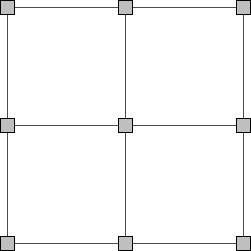
\includegraphics[height=0.7\textheight]{../figs/PuestaTierra.pdf}
\end{center}
\end{frame}

\begin{frame}[label={sec:orgae98c9b}]{Ejemplo}
\begin{itemize}
\item En primer lugar calculamos la resistencia aportada por el conductor enterrado:
\end{itemize}
\begin{align*}
  L_c &= 4 \cdot 2 \cdot 6 = \qty{48}{\meter}\\
  R_{tc} &= \frac{2\rho}{L_c} = \qty{8.75}{\ohm}
\end{align*}
\begin{itemize}
\item La resistencia de una pica vertical de \(\qty{2}{\meter}\) con este terreno es de:
\end{itemize}
\begin{equation*}
  R_{tp} = \frac{\rho}{L_p} = \qty{105}{\ohm}
\end{equation*}

\begin{itemize}
\item Por tanto, el número total de picas necesarias es:
\end{itemize}
\begin{equation*}
  \frac{1}{5} =\frac{n_p}{105} + \frac{1}{8.75} \rightarrow n_p = 9
\end{equation*}
\end{frame}
\end{document}